\section{From Sputnik to Apollo 11}

\subsection{Early Soviet lead}
This section discusses early soviet lead during the Moon Race.

Both superpowers linked orbital achievements to national prestige. \cite{siddiqi2010}

\subsection{US lunar landing}
This section discusses us lunar landing during the Moon Race.

Both superpowers linked orbital achievements to national prestige. \cite{siddiqi2010}

\begin{figure}[htbp]
\centering
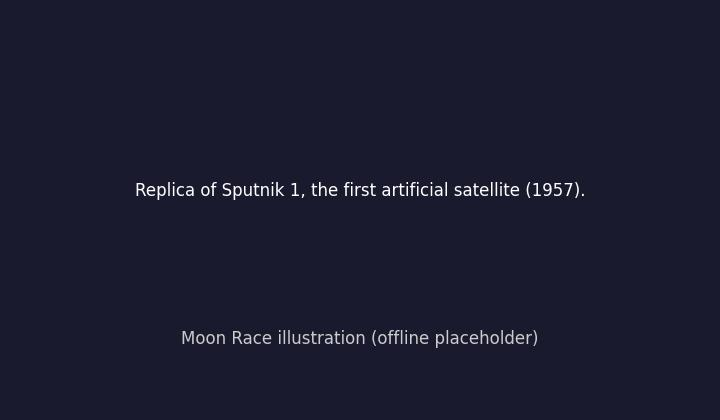
\includegraphics[width=0.88\linewidth]{figures/ch02_sputnik.jpg}
\caption{Sputnik era - the Soviet Union launched the first artificial satellite in 1957.}
\label{fig:ch_sputnik_era_the_soviet_union_lau}
\end{figure}

\bigskip
\begin{otherlanguage}{hebrew}
\subsection*{סיכום הפרק}

פרק זה עוסק ביתרון הסובייטי המוקדם: שיגור הלוויין הראשון והטסת האדם הראשון לחלל. הישגים אלו זעזעו את ארצות הברית והאיצו את תגובתה.

\end{otherlanguage}

\clearpage
